\documentclass{beamer}

\usepackage{comment}
\usepackage{color}

\title{Unstructured Grids}
\author{Glenn Hammond}
\date{\today}

\begin{document}
  
\frame{\titlepage}


\subsection{Type of Unstructured Grids}

\begin{frame}[fragile]\frametitle{Types of Unstructured  Grids}

\begin{itemize}
  \item UNSTRUCTURED
  \begin{itemize}
     \item PFLOTRAN Jargon: Unstructured Implicit (.ugi)
     \item Finite element approach (cells and vertices)
     \item Cell are defined by a list of vertices.
     \item Vertices are define by coordinates.
   \end{itemize}
  \item UNSTRUCTURED\_EXPLICIT
  \begin{itemize}
     \item PFLOTRAN Jargon: Unstructured Explicit (.uge)
    \item Used for Voronoi-style grids that list explicit connectivity
    \item Cells are defined with an ID, coordinate, and volume.
    \item Connections are defined with two grid cell IDs (one on either side of the connection), a coordinate for the intersection with the face and an area.
  \end{itemize}
\end{itemize}

\end{frame}

\begin{frame}[fragile]\frametitle{UNSTRUCTURED (Finite Element)}
\vspace{0.2in}
\centering
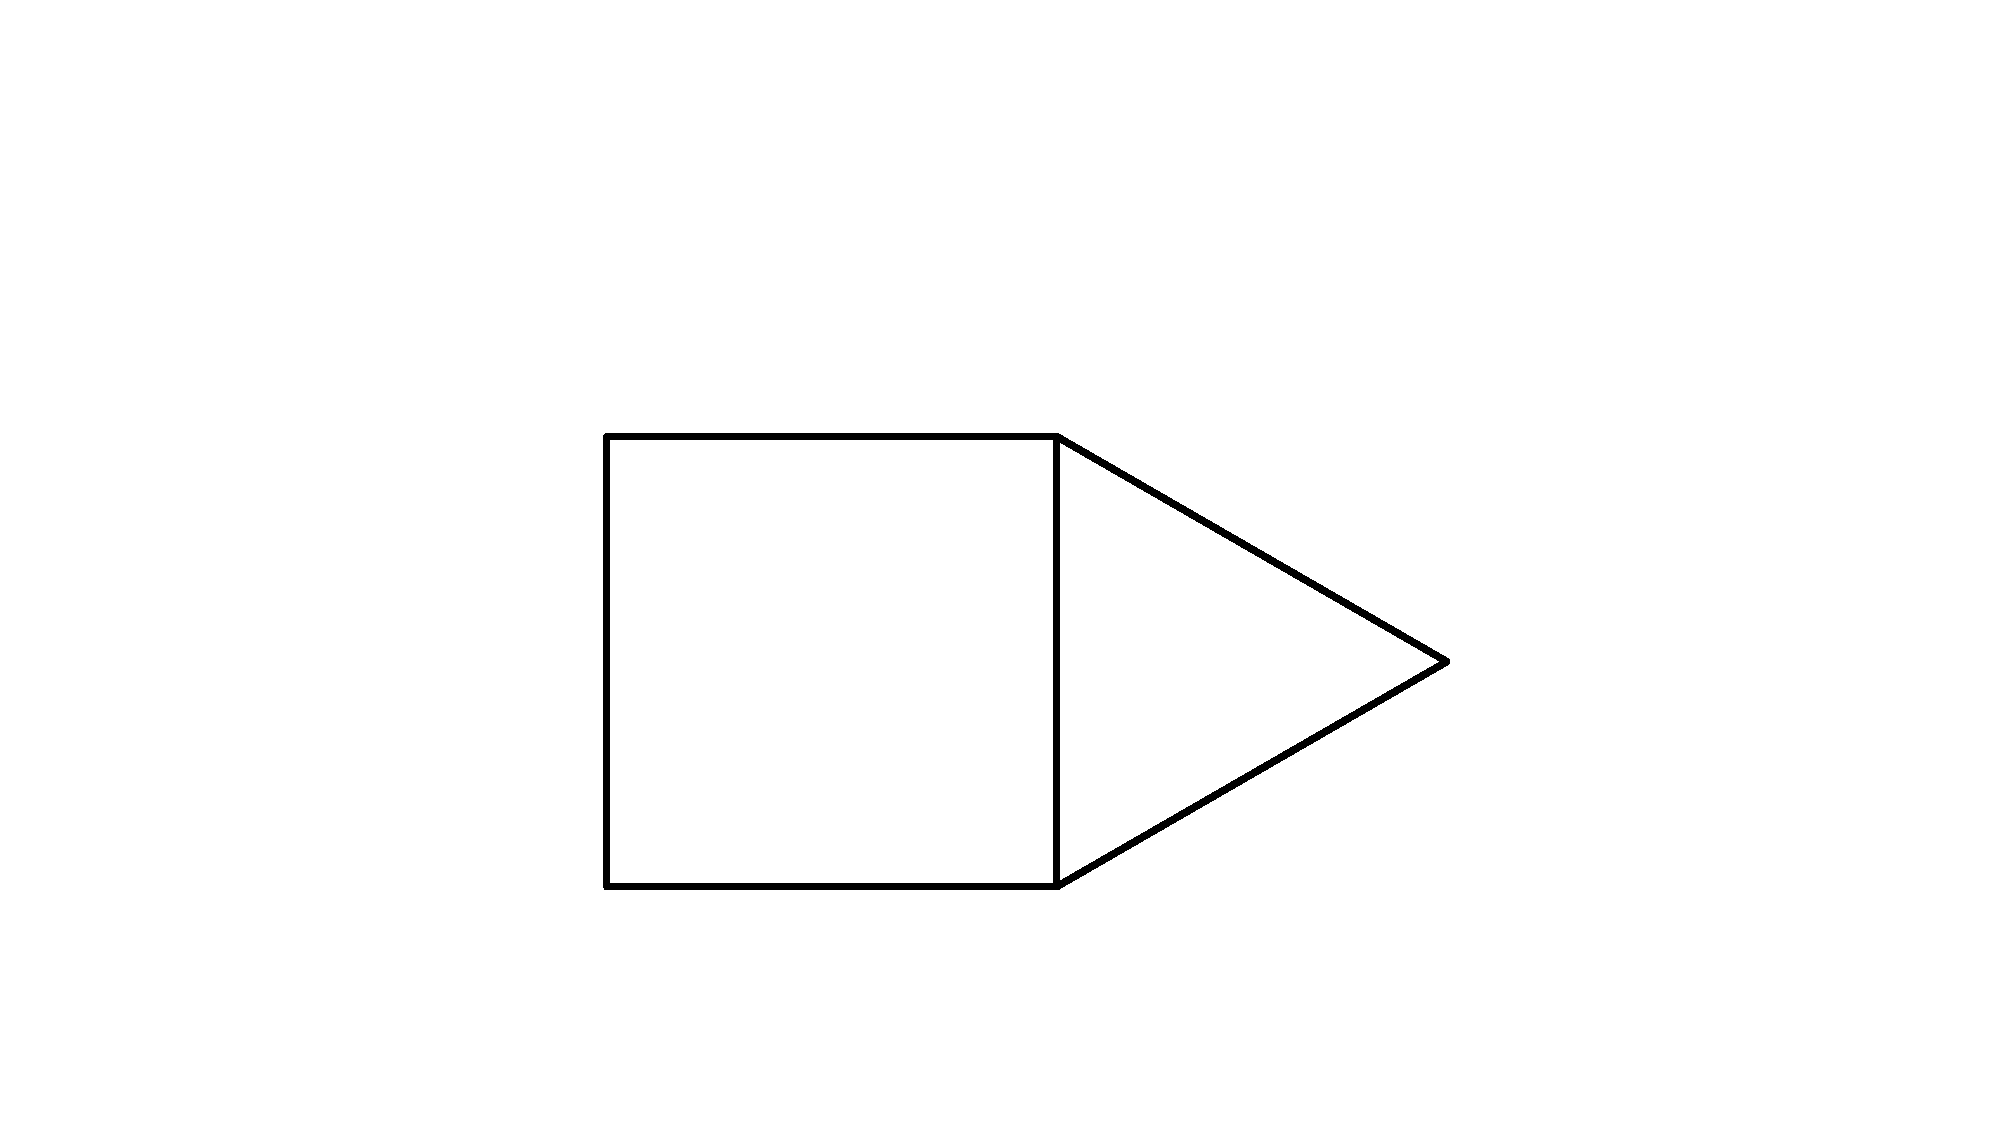
\includegraphics[width=1\linewidth]{./fe_geom}
\end{frame}


\begin{frame}[fragile]\frametitle{UNSTRUCTURED (Finite Element)}
\vspace{0.2in}
\centering
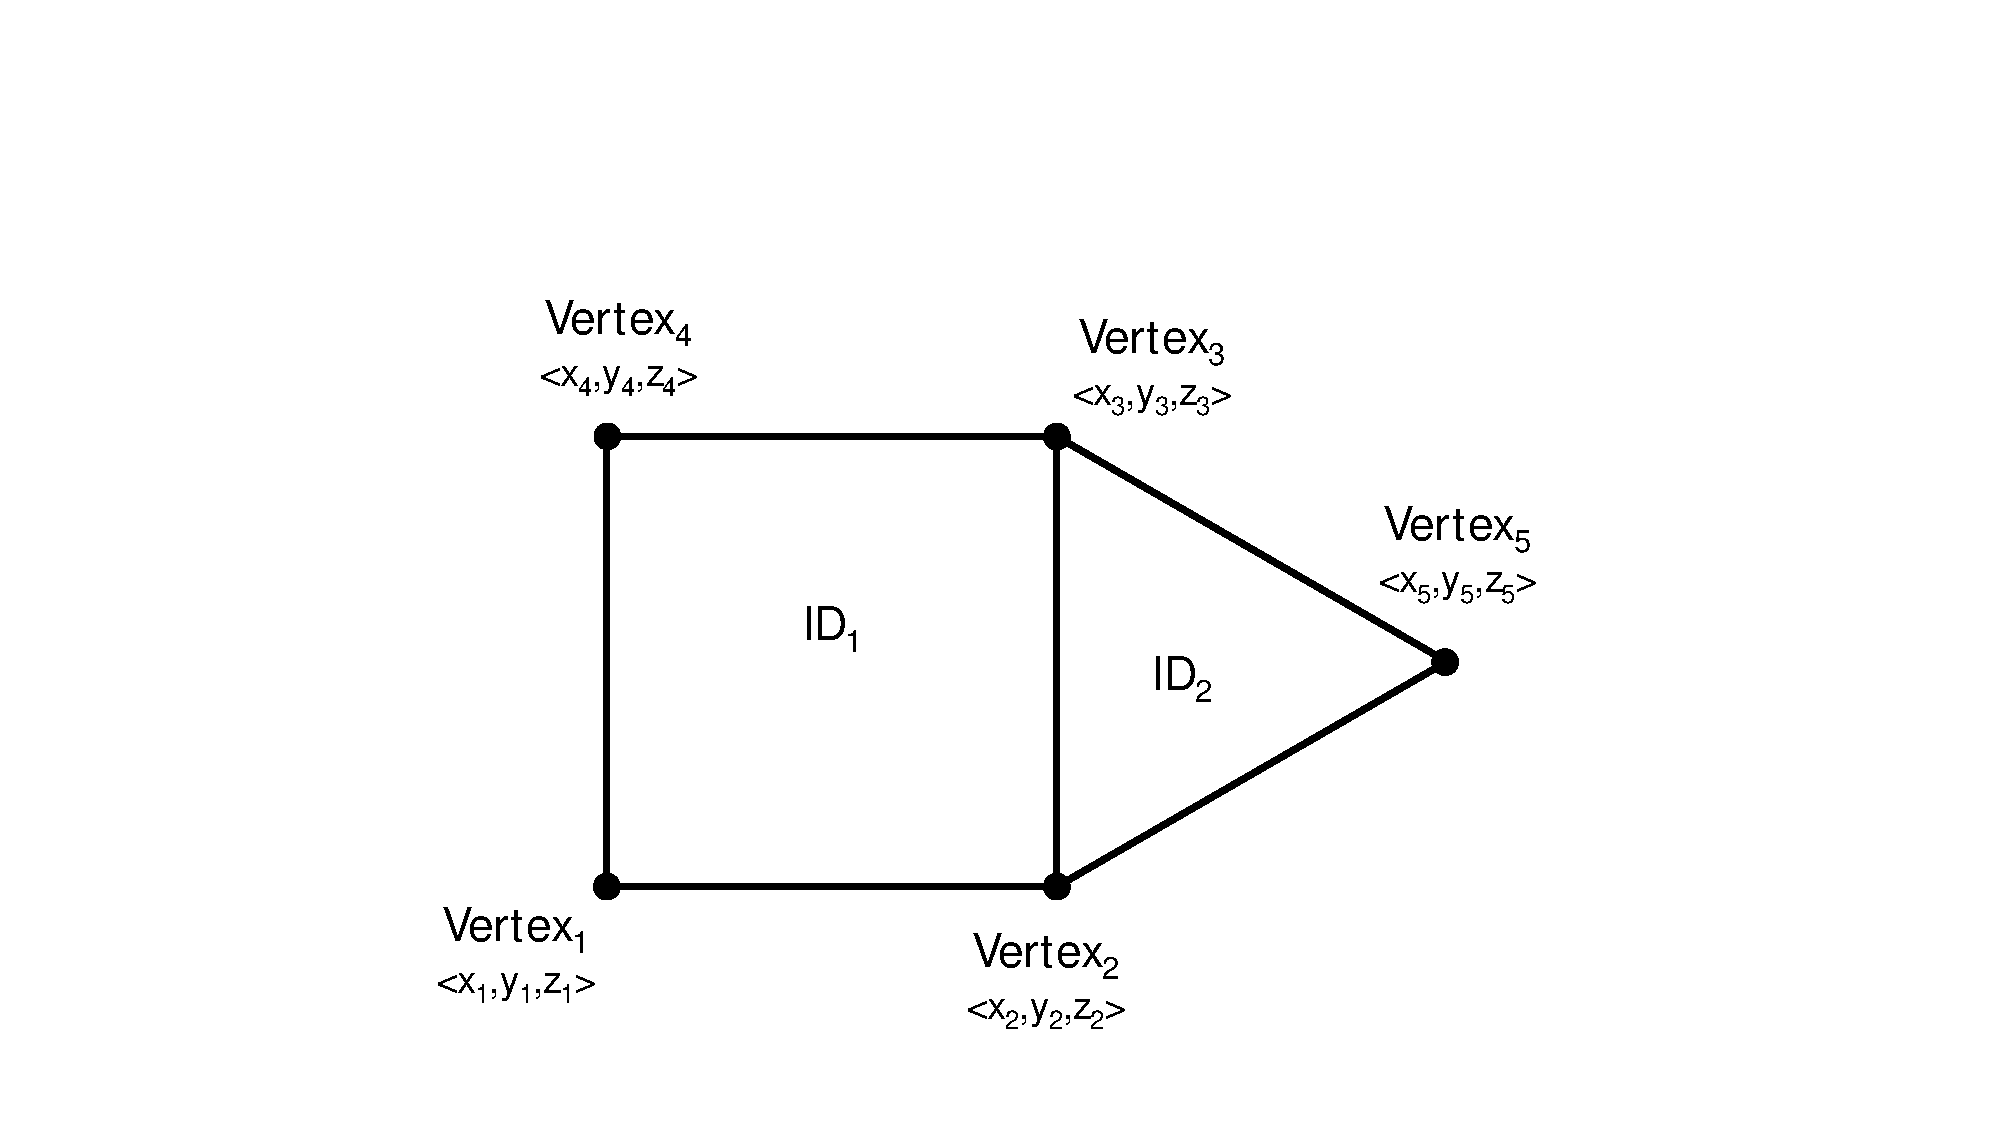
\includegraphics[width=1\linewidth]{./fe_raw}
\end{frame}

\begin{frame}[fragile,containsverbatim]\frametitle{UNSTRUCTURED (File Format)}
.ugi file format:
\small
\begin{semiverbatim}
  NUM_CELLS NUM_VERTICES
  CELL_TYPE VERTEX_1 VERTEX_2 ... VERTEX_N
  ...
  CELL_TYPE VERTEX_1 VERTEX_2 ... VERTEX_N
  VERTEX_X_COORDINATE VERTEX_Y_COORDINATE VERTEX_Z_COORDINATE
  ...
  VERTEX_X_COORDINATE VERTEX_Y_COORDINATE VERTEX_Z_COORDINATE
\end{semiverbatim}

Cell Types:
\begin{itemize}
  \item T - tetrahedron (4 vertices)
  \item P - pyramid (5 vertices)
  \item W - wedge (6 vertices)
  \item H - hexahedron (8 vertices)
\end{itemize}
\end{frame}

\begin{frame}[fragile,containsverbatim]\frametitle{UNSTRUCTURED (File Example)}

\begin{minipage}[t]{0.48\linewidth}
\vspace{0.2in}
.ugi file contents
\begin{semiverbatim}
  2 5
  Q 1 2 3 4
  T 2 5 3
  x1 y1 z1
  x2 y2 z2
  x3 y3 z3
  x4 y4 z4
  x5 y5 z5
\end{semiverbatim}
\scriptsize
\vspace{0.1in}
\textit{Q is quadrilateral and T is triangle for demonstration only. 2D cells are not supported in PFLOTRAN.}
\end{minipage}
\hfill
\begin{minipage}[t]{0.48\linewidth}
\vspace{0.01in}
\hspace{-.75in}
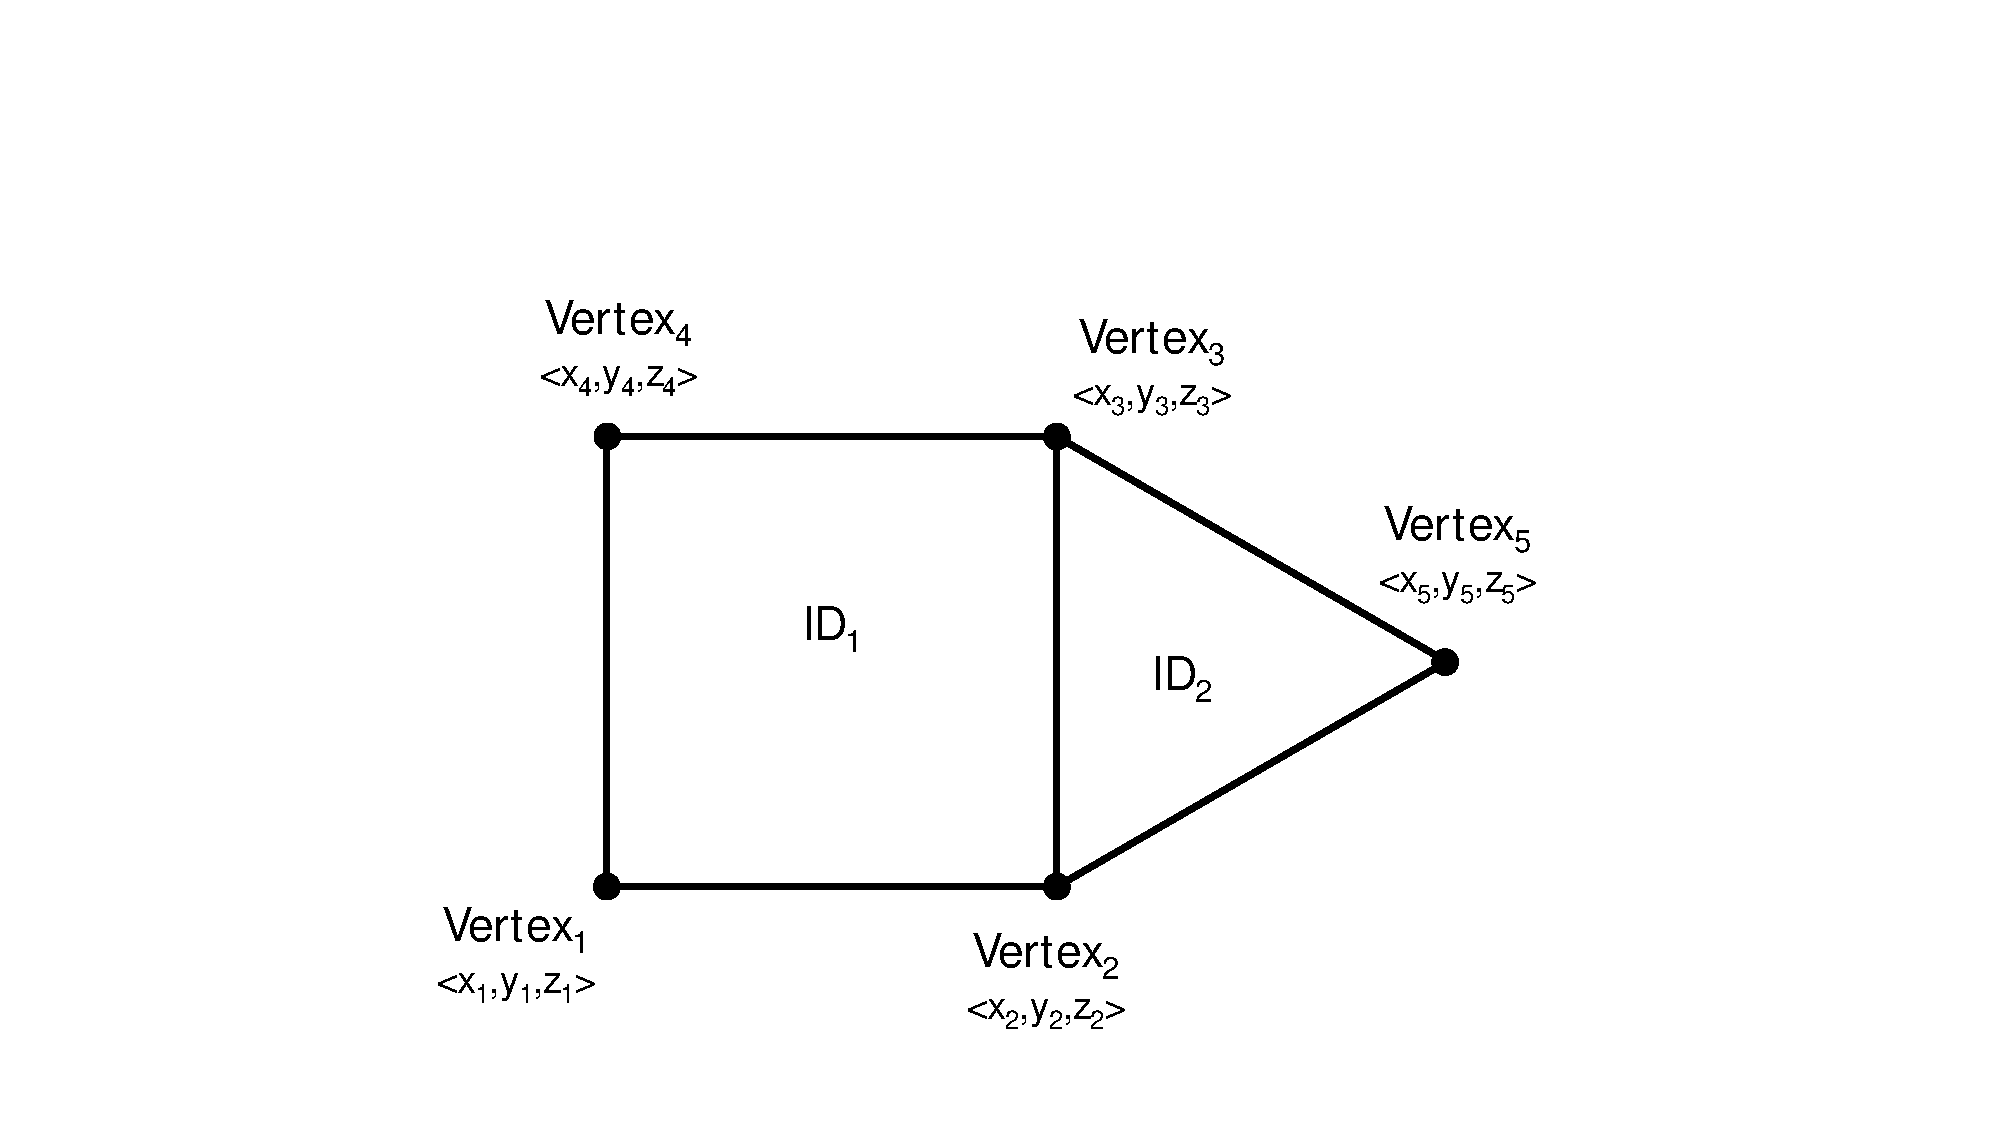
\includegraphics[width=1.5\linewidth]{./fe_raw}
\end{minipage}

\end{frame}


\begin{frame}[fragile]\frametitle{UNSTRUCTURED (Finite Element + Dual)}
Centroids, distances, areas and volumes are calculated internally.
\vspace{0.2in}
\centering
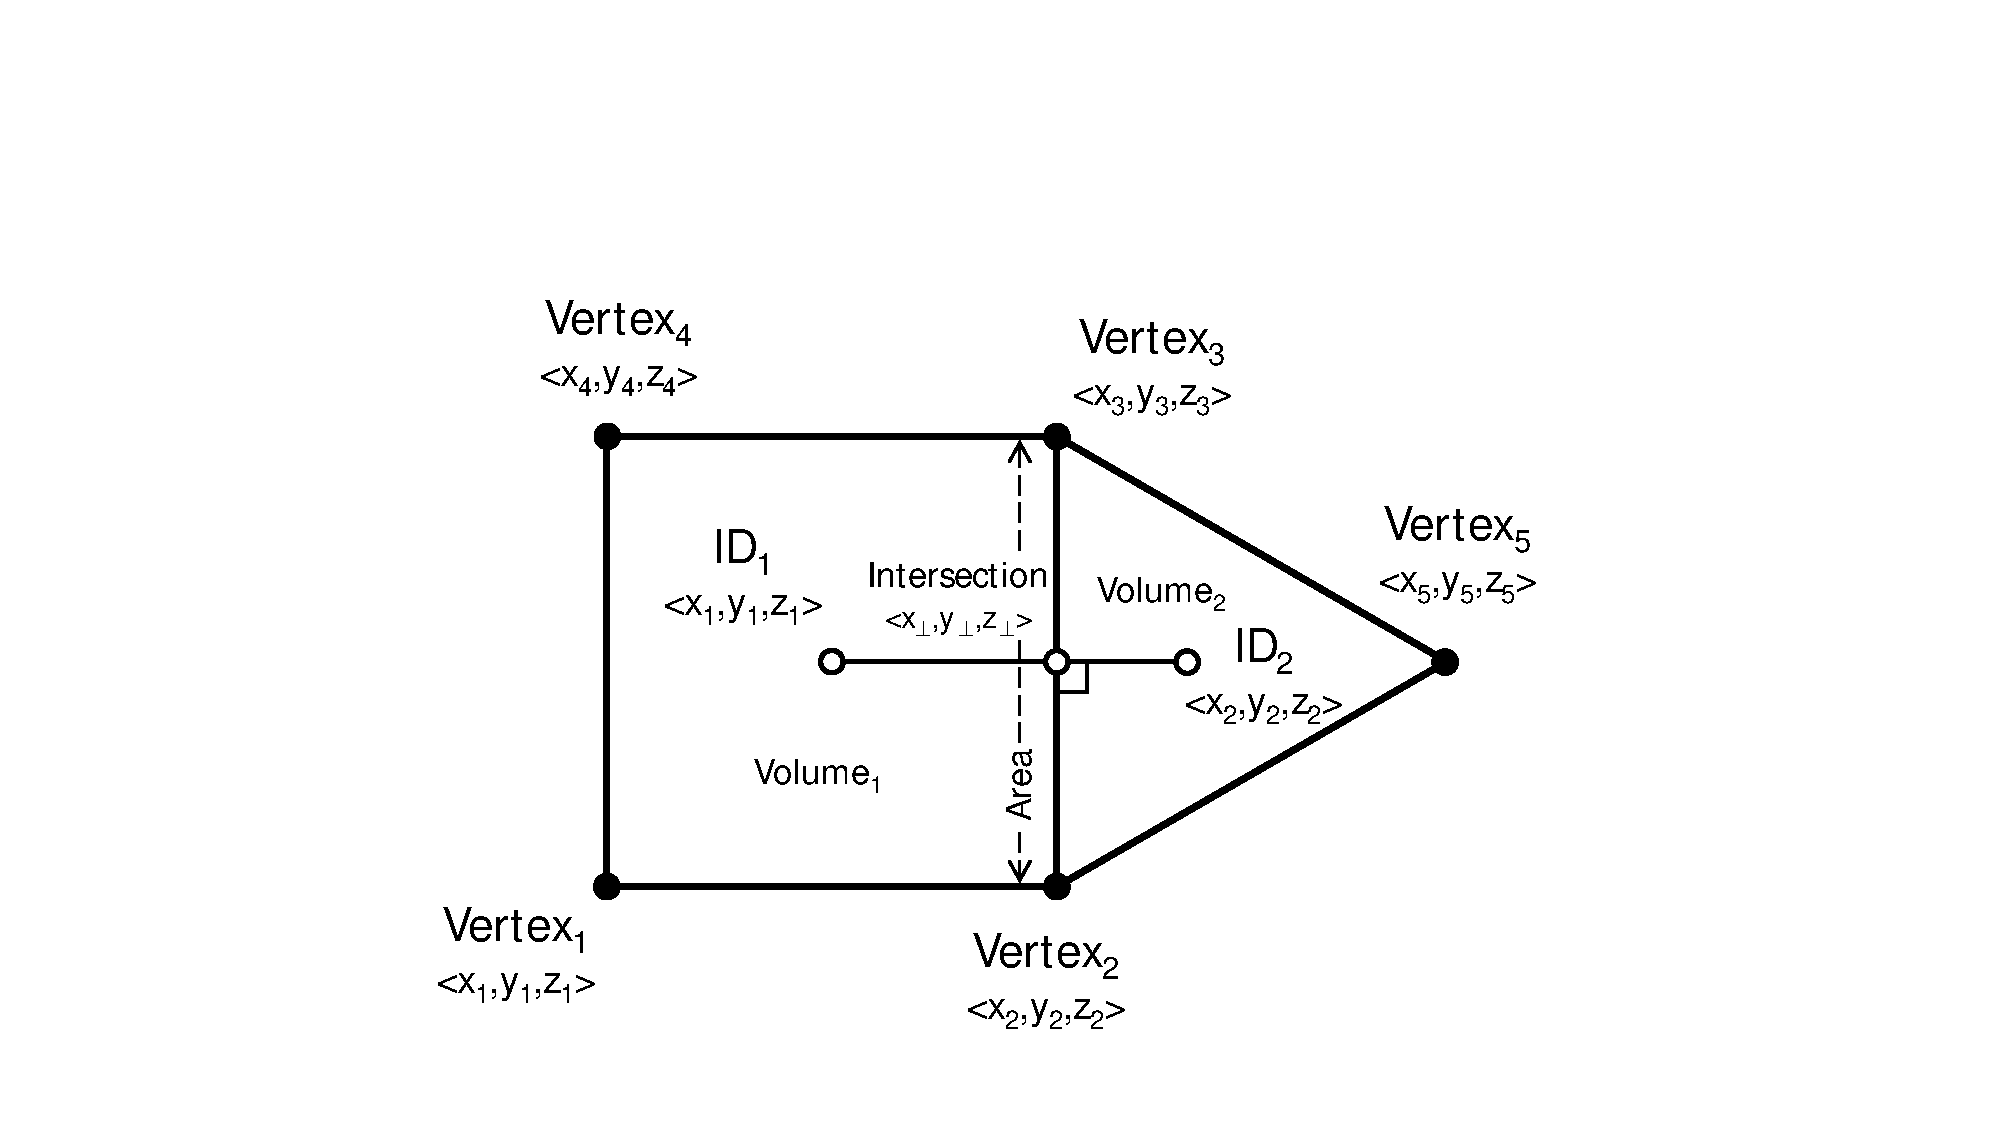
\includegraphics[width=1\linewidth]{./fe_all}
\end{frame}

\begin{frame}[fragile]\frametitle{UNSTRUCTURED (Dual)}
\vspace{0.2in}
\centering
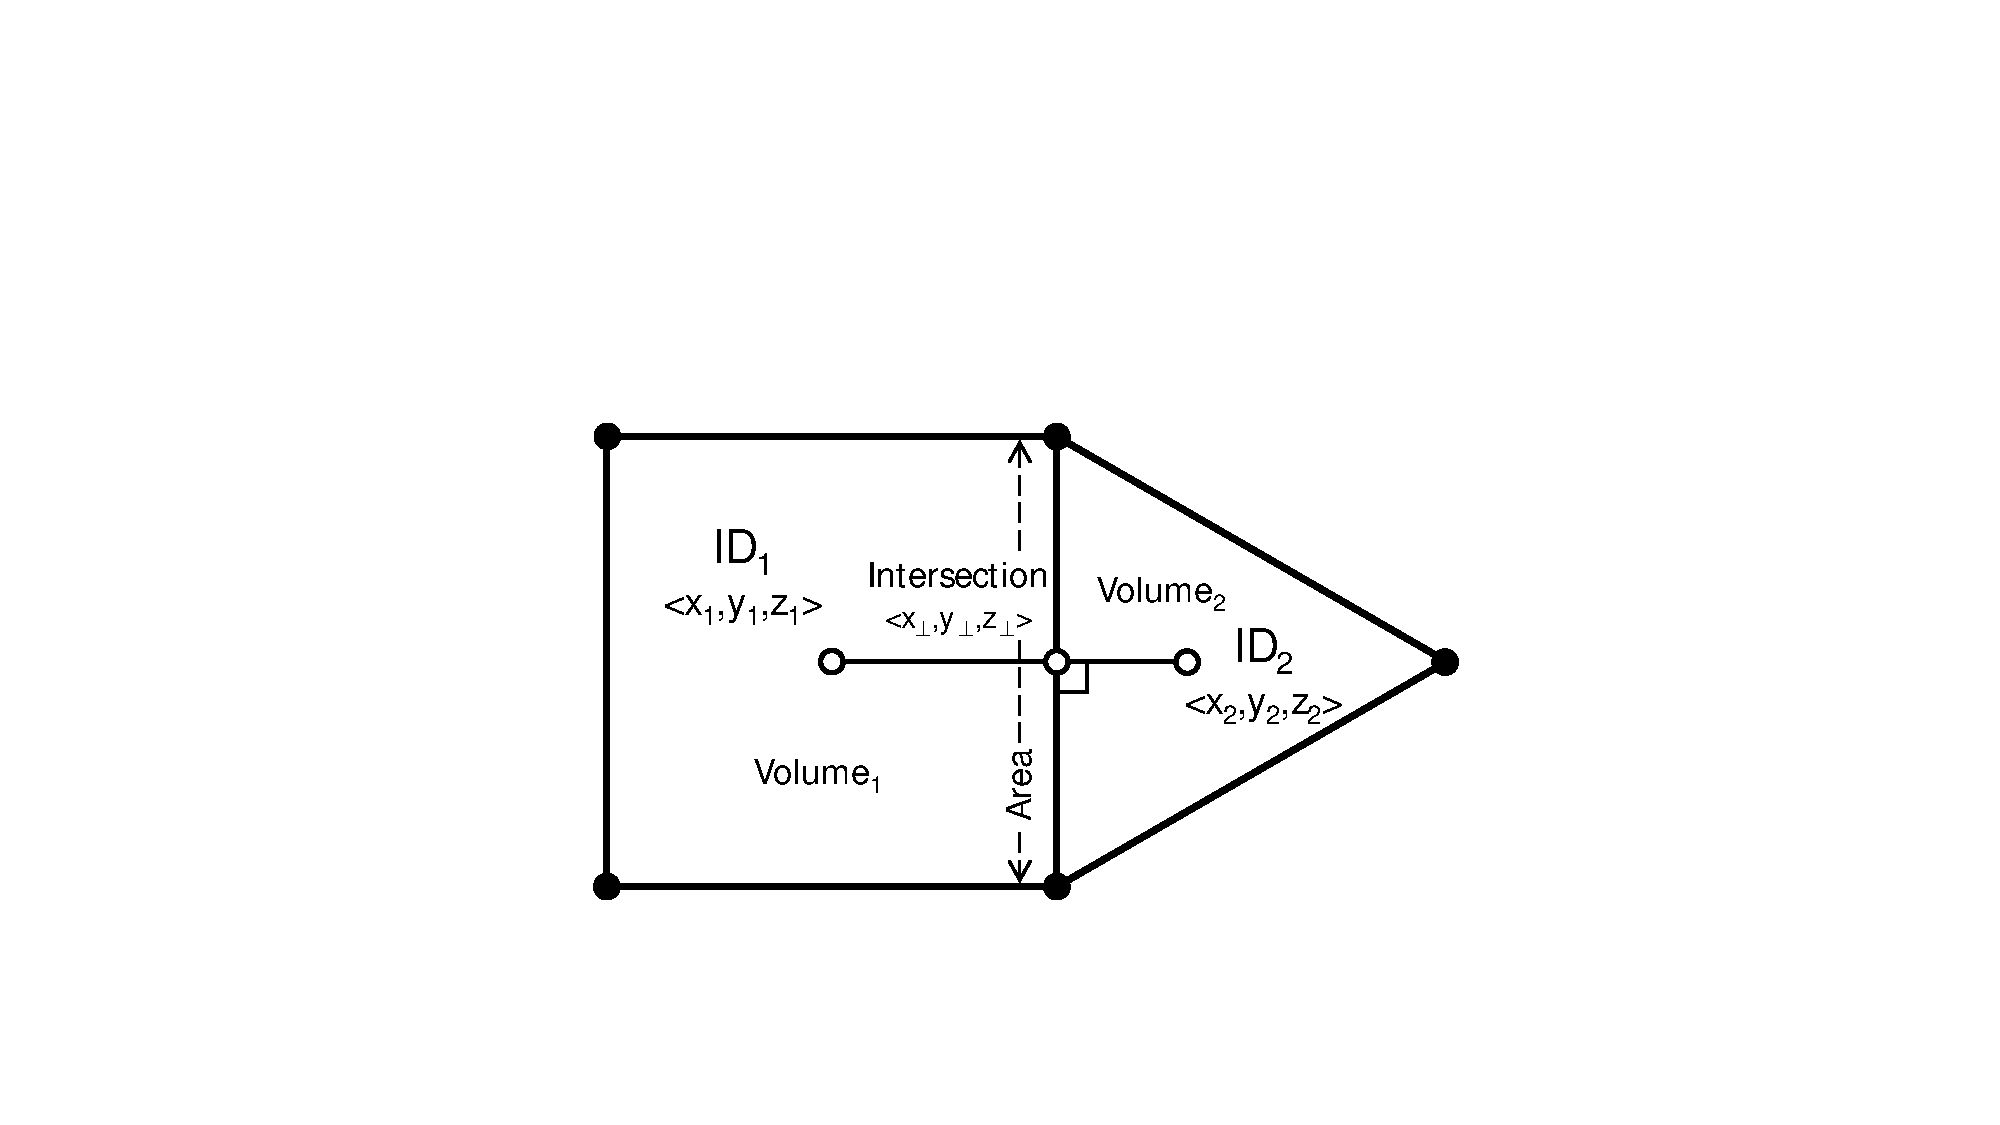
\includegraphics[width=1\linewidth]{./fe_dual}
\end{frame}

\begin{frame}[fragile]\frametitle{UNSTRUCTURED (Distorted)}
\vspace{0.2in}
\centering
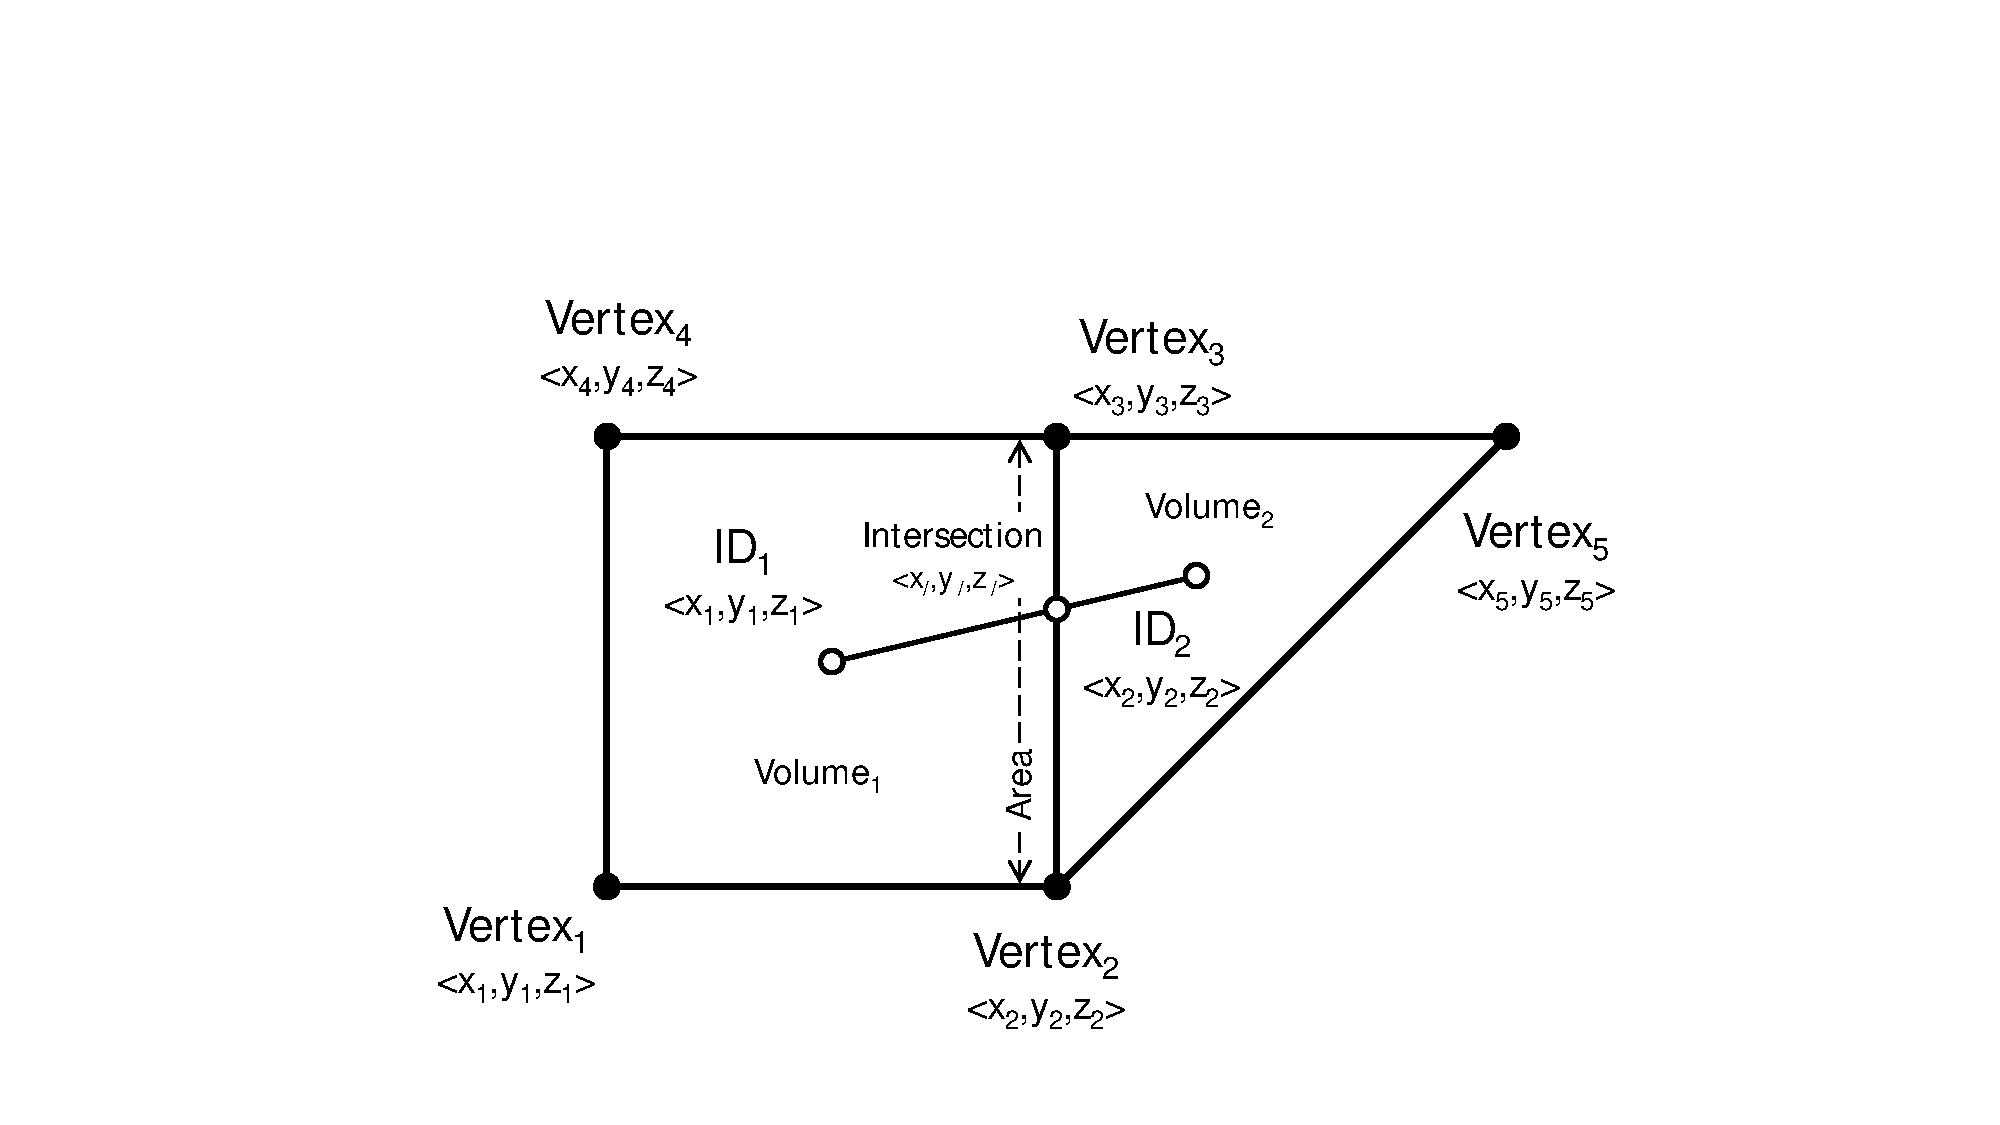
\includegraphics[width=1\linewidth]{./fe_distort_all}
\end{frame}

\begin{frame}[fragile]\frametitle{UNSTRUCTURED (Distorted Dual)}
\vspace{0.2in}
\centering
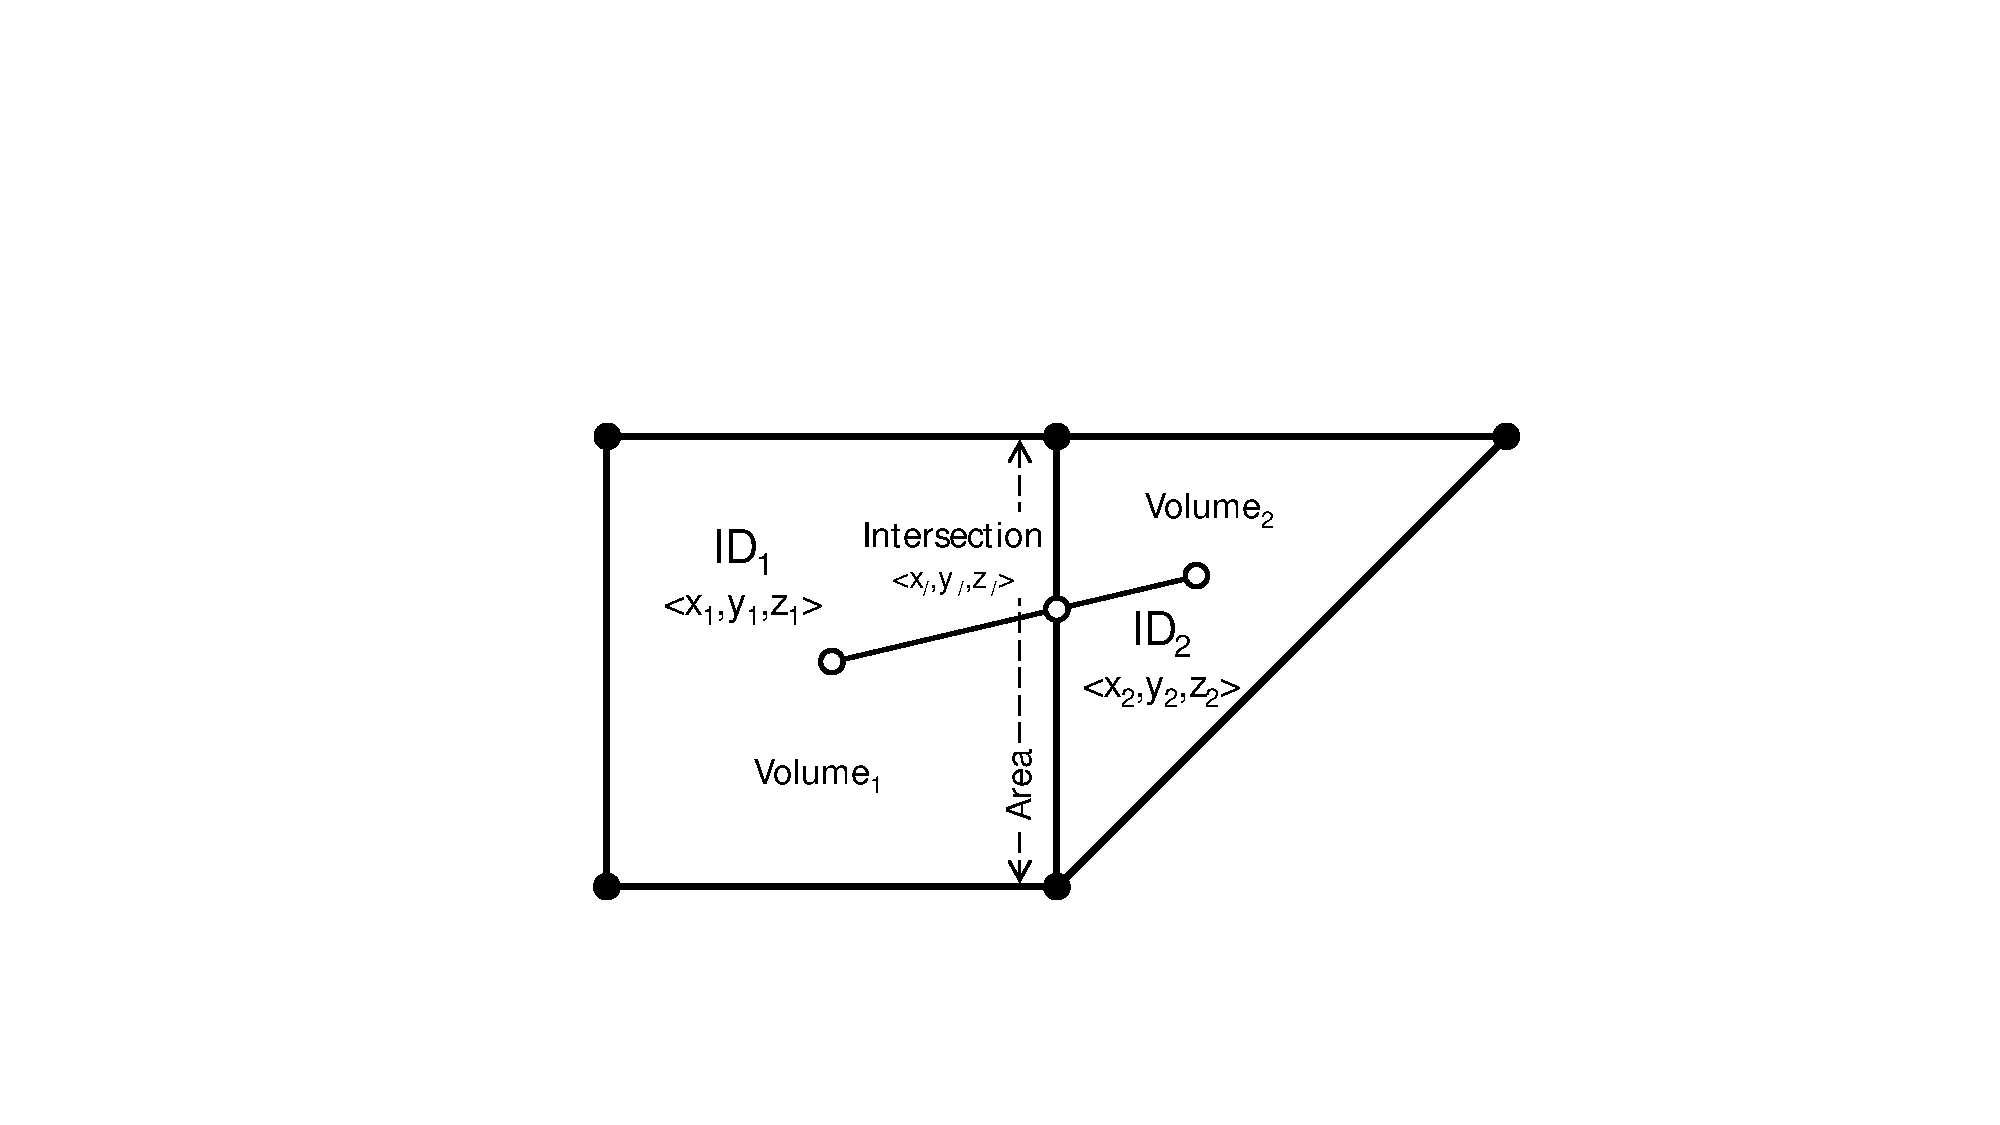
\includegraphics[width=1\linewidth]{./fe_distort_dual}
\end{frame}

\begin{frame}[fragile]\frametitle{UNSTRUCTURED\_EXPLICIT}
\vspace{0.2in}
\centering
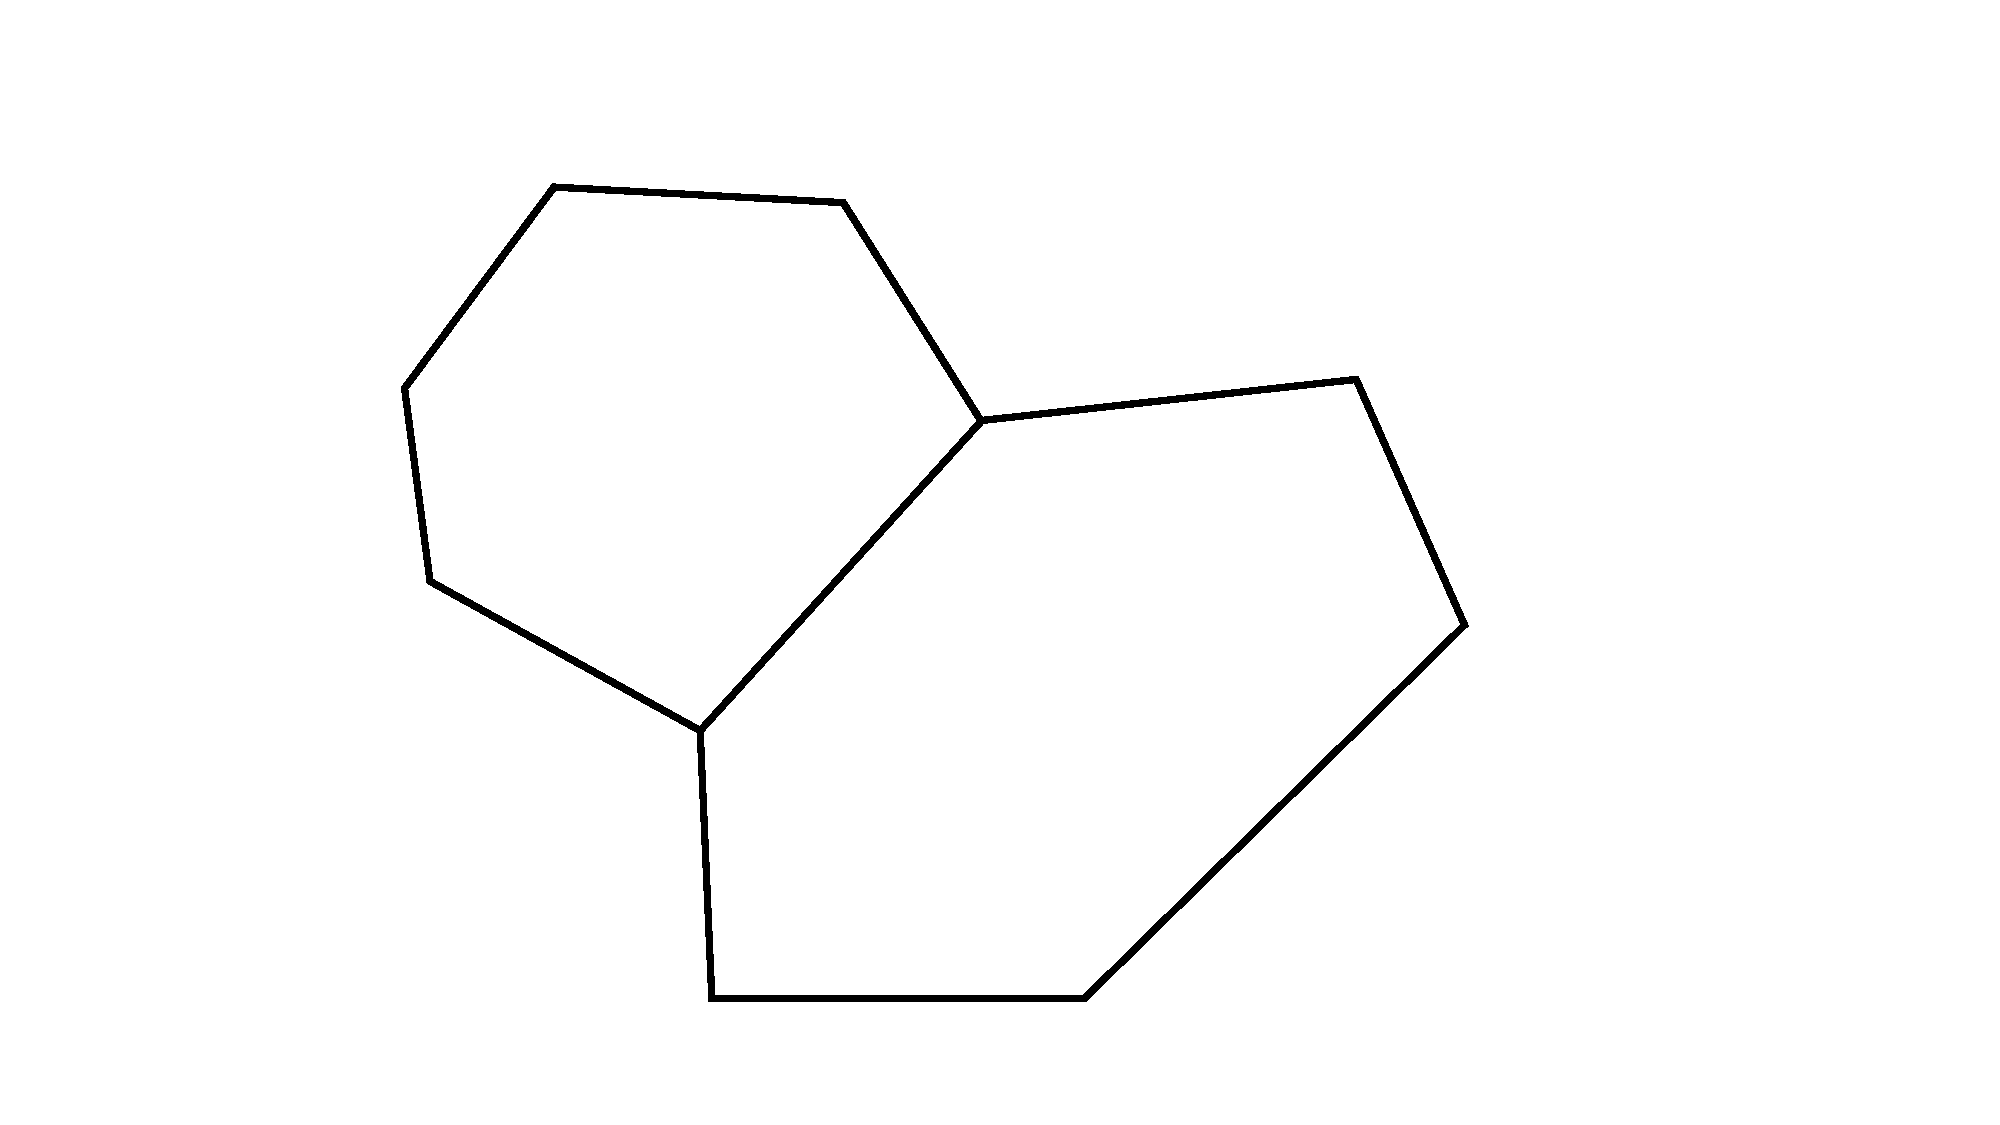
\includegraphics[width=0.9\linewidth]{./voronoi_geom}
\end{frame}

\begin{frame}[fragile,containsverbatim]\frametitle{UNSTRUCTURED\_EXPLICIT (File Format)}
.uge file format:
\begin{semiverbatim}
CELLS #
1 X\_coordinate Y\_coordinate Z\_coordinate VOLUME
...
# X\_coordinate Y\_coordinate Z\_coordinate VOLUME
CONNECTIONS #
CELL\_a CELL\_b X\_coordinate Y\_coordinate Z\_coordinate AREA
...
CELL\_y CELL\_z X\_coordinate Y\_coordinate Z\_coordinate AREA
\end{semiverbatim}

\end{frame}

\begin{frame}[fragile]\frametitle{UNSTRUCTURED\_EXPLICIT}
\vspace{0.2in}
\centering
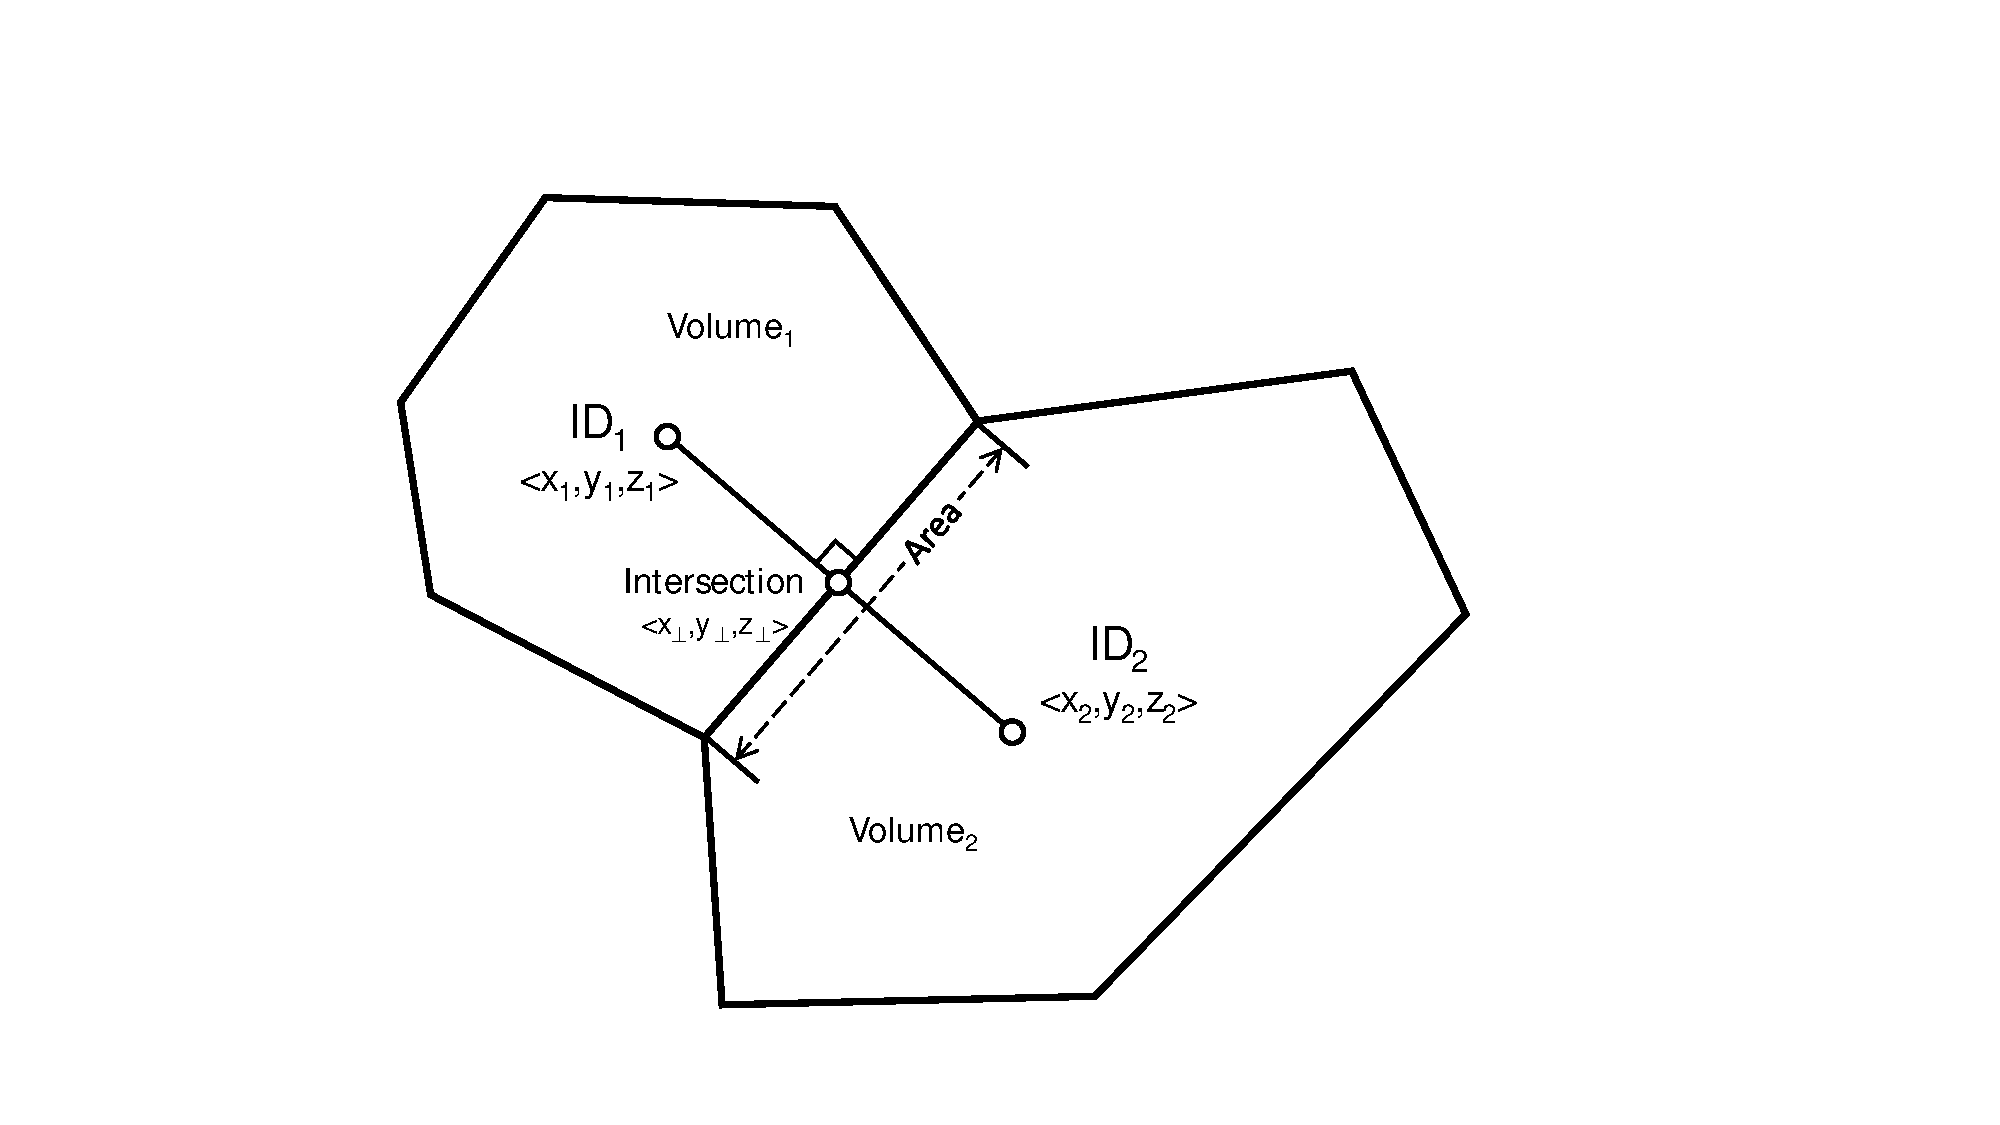
\includegraphics[width=0.9\linewidth]{./voronoi_dual}
\end{frame}


\begin{frame}[fragile,containsverbatim]\frametitle{UNSTRUCTURED\_EXPLICIT (File Example)}

\begin{minipage}[t]{0.48\linewidth}
\vspace{0.4in}
.uge file contents
\begin{semiverbatim}
CELLS 2
1 x1 y1 z1 Volume1
2 x2 y2 z2 Volume2
CONNECTIONS 1
1 2 x| y| z| Area
\end{semiverbatim}
\end{minipage}
\hfill
\begin{minipage}[t]{0.48\linewidth}
\vspace{0.01in}
\hspace{-.5in}
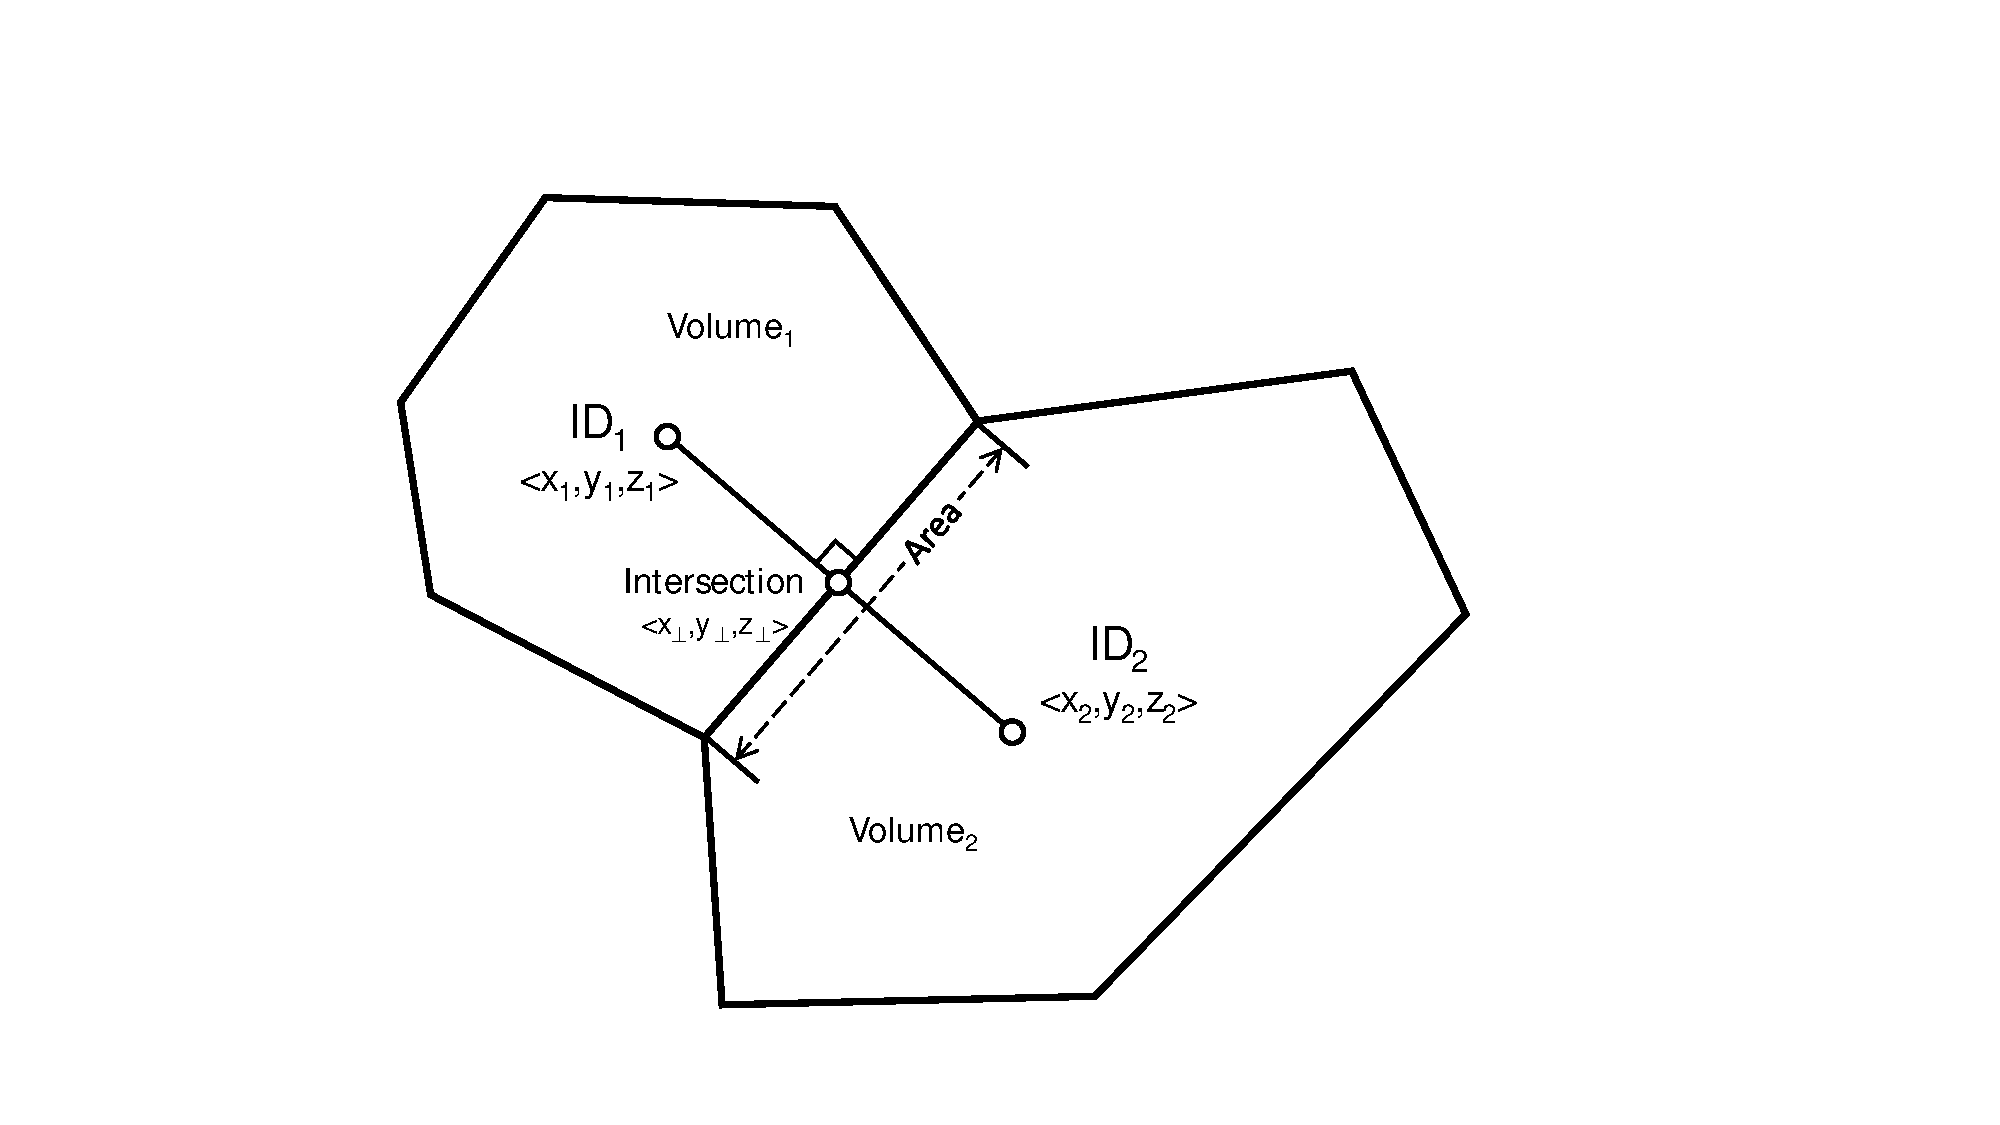
\includegraphics[width=1.3\linewidth]{./voronoi_dual}
\end{minipage}

\end{frame}


\end{document}
